\documentclass[tikz,border=2pt]{standalone}
\usepackage{mathptmx}
\usepackage{amsmath}
\usetikzlibrary{arrows.meta,calc,backgrounds}

% A single-column, editable vector motivating example.
% All domains and AS labels are illustrative; no geography is implied.
\definecolor{pvblue}{HTML}{0072B2}
\definecolor{pvgreen}{HTML}{009E73}
\definecolor{pvgray}{HTML}{5F6670}

\begin{document}
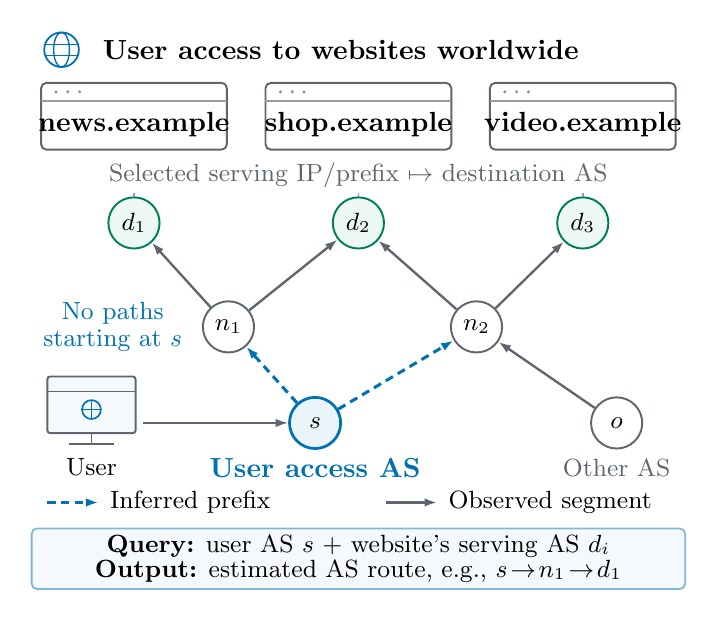
\begin{tikzpicture}[
  font=\fontsize{8.8}{10}\selectfont,
  >={Latex[length=1.6mm,width=1.1mm]},
  as/.style={circle,draw=pvgray,line width=.7pt,fill=white,
             minimum size=6.5mm,inner sep=0pt},
  endpoint/.style={as,draw=pvgreen!80!black,fill=pvgreen!7},
  observed/.style={->,draw=pvgray,line width=.85pt},
  inferred/.style={->,draw=pvblue,dash pattern=on 3pt off 2pt,line width=1.1pt},
  association/.style={draw=pvgray!65,line width=.55pt},
  note/.style={align=center,inner sep=0pt}
]
\path[use as bounding box] (0,0) rectangle (8.4,7.15);

% A globe denotes worldwide website choice, not a geographical route.
\begin{scope}[shift={(.43,6.87)}]
  \draw[pvblue,line width=.65pt] (0,0) circle (.22);
  \draw[pvblue,line width=.5pt] (0,0) ellipse (.10 and .22);
  \draw[pvblue,line width=.5pt] (-.21,.07)--(.21,.07) (-.21,-.07)--(.21,-.07);
\end{scope}
\node[anchor=west,font=\bfseries\fontsize{10.2}{11.2}\selectfont]
  at (.83,6.87) {User access to websites worldwide};

% Browser cards identify Web destinations, using reserved example names.
\foreach \x/\domain/\kind in {
  1.35/news.example/News,
  4.20/shop.example/Shopping,
  7.05/video.example/Video} {
  \draw[rounded corners=2pt,draw=pvgray,fill=white,line width=.7pt]
    (\x-1.18,5.60) rectangle (\x+1.18,6.45);
  \draw[draw=pvgray!65,line width=.5pt]
    (\x-1.18,6.22)--(\x+1.18,6.22);
  \foreach \dx in {-.99,-.84,-.69}
    \fill[pvgray!70] (\x+\dx,6.335) circle (.022);
  \node[note,font=\bfseries] at (\x,5.92) {\domain};
}

\node[note,text=pvgray] at (4.2,5.27)
  {Selected serving IP/prefix $\mapsto$ destination AS};
\node[endpoint] (d1) at (1.35,4.67) {$d_1$};
\node[endpoint] (d2) at (4.20,4.67) {$d_2$};
\node[endpoint] (d3) at (7.05,4.67) {$d_3$};
\draw[association] (d1.north)--(1.35,5.05);
\draw[association] (d2.north)--(4.20,5.05);
\draw[association] (d3.north)--(7.05,5.05);

% Indirect evidence is visible, but the user's outbound choices are not.
\node[as] (n) at (2.55,3.35) {$n_1$};
\node[as] (a) at (5.70,3.35) {$n_2$};
\node[as] (o) at (7.48,2.13) {$o$};
\node[note,text=pvgray,anchor=north] at (7.48,1.68) {Other AS};
\draw[observed] (o)--(a);
\draw[observed] (a)--(d2);
\draw[observed] (a)--(d3);
\draw[observed] (n)--(d2);
\draw[observed] (n)--(d1);

\node[as,draw=pvblue,fill=pvblue!8,line width=1pt] (s) at (3.65,2.13) {$s$};
\draw[inferred] (s)--(n);
\draw[inferred] (s)--(a);
\node[note,text=pvblue,anchor=north,font=\bfseries] at (3.65,1.68) {User access AS};

% User/browser icon, separate from the inferred interdomain route.
\draw[rounded corners=1pt,draw=pvgray,line width=.7pt,fill=pvblue!4]
  (.25,2.00) rectangle (1.37,2.72);
\draw[draw=pvgray,line width=.6pt] (.25,2.53)--(1.37,2.53);
\draw[draw=pvgray,line width=.6pt] (.81,2.00)--(.81,1.86) (.53,1.86)--(1.09,1.86);
\draw[pvblue,line width=.6pt] (.81,2.30) circle (.12);
\draw[pvblue,line width=.6pt] (.69,2.30)--(.93,2.30) (.81,2.18)--(.81,2.42);
\node[note,anchor=north] at (.81,1.68) {User};
\draw[->,draw=pvgray,line width=.7pt] (1.47,2.13)--(s.west);
\node[note,text width=2.05cm,text=pvblue] at (1.08,3.35)
  {No paths\\starting at $s$};

% Line style carries meaning independently of color.
\draw[inferred] (.25,1.12)--(.90,1.12);
\node[anchor=west,inner sep=0pt] at (1.04,1.12) {Inferred prefix};
\draw[observed] (4.55,1.12)--(5.20,1.12);
\node[anchor=west,inner sep=0pt] at (5.34,1.12) {Observed segment};

\draw[rounded corners=2pt,draw=pvblue!50,fill=pvblue!4,line width=.65pt]
  (.05,.02) rectangle (8.35,.79);
\node[note] at (4.2,.57)
  {\textbf{Query:} user AS $s$ + website's serving AS $d_i$};
\node[note] at (4.2,.25)
  {\textbf{Output:} estimated AS route, e.g., $s\!\to\!n_1\!\to\!d_1$};

\end{tikzpicture}
\end{document}
